
\documentclass[11pt,pressrelease]{newlfm} % Font size

\usepackage{charter} % Use the Charter font for the document text

\PhrContact{Team name} % Uncomment this line to change the 'Contact:' text

\makeletterhead{Uiuc}{\Cheader{\vspace{16pt}
\includegraphics[width=0.5\linewidth]{logo.png}}} % Include a company logo, if you don't use one you will need to uncomment line 6 in the prsrls.tex file
\lthUiuc % Print the company/institution logo

\release{Subtrop Harvest Application} % When the press release may be used
%
\namefrom{Brute Force} % Name


\headline{Project Tender} % Headline for the press release

\newcommand{\subtitle}{} % Subtitle for the press release, if you don't want one just remove the subtitle text leaving the rest of the command


%----------------------------------------------------------------------------------------

\begin{document}
\begin{newlfm}

%----------------------------------------------------------------------------------------
%	PRESS RELEASE CONTENT
%----------------------------------------------------------------------------------------

\begin{singlespace} % Uncomment for single line spacing

\begin{center}
	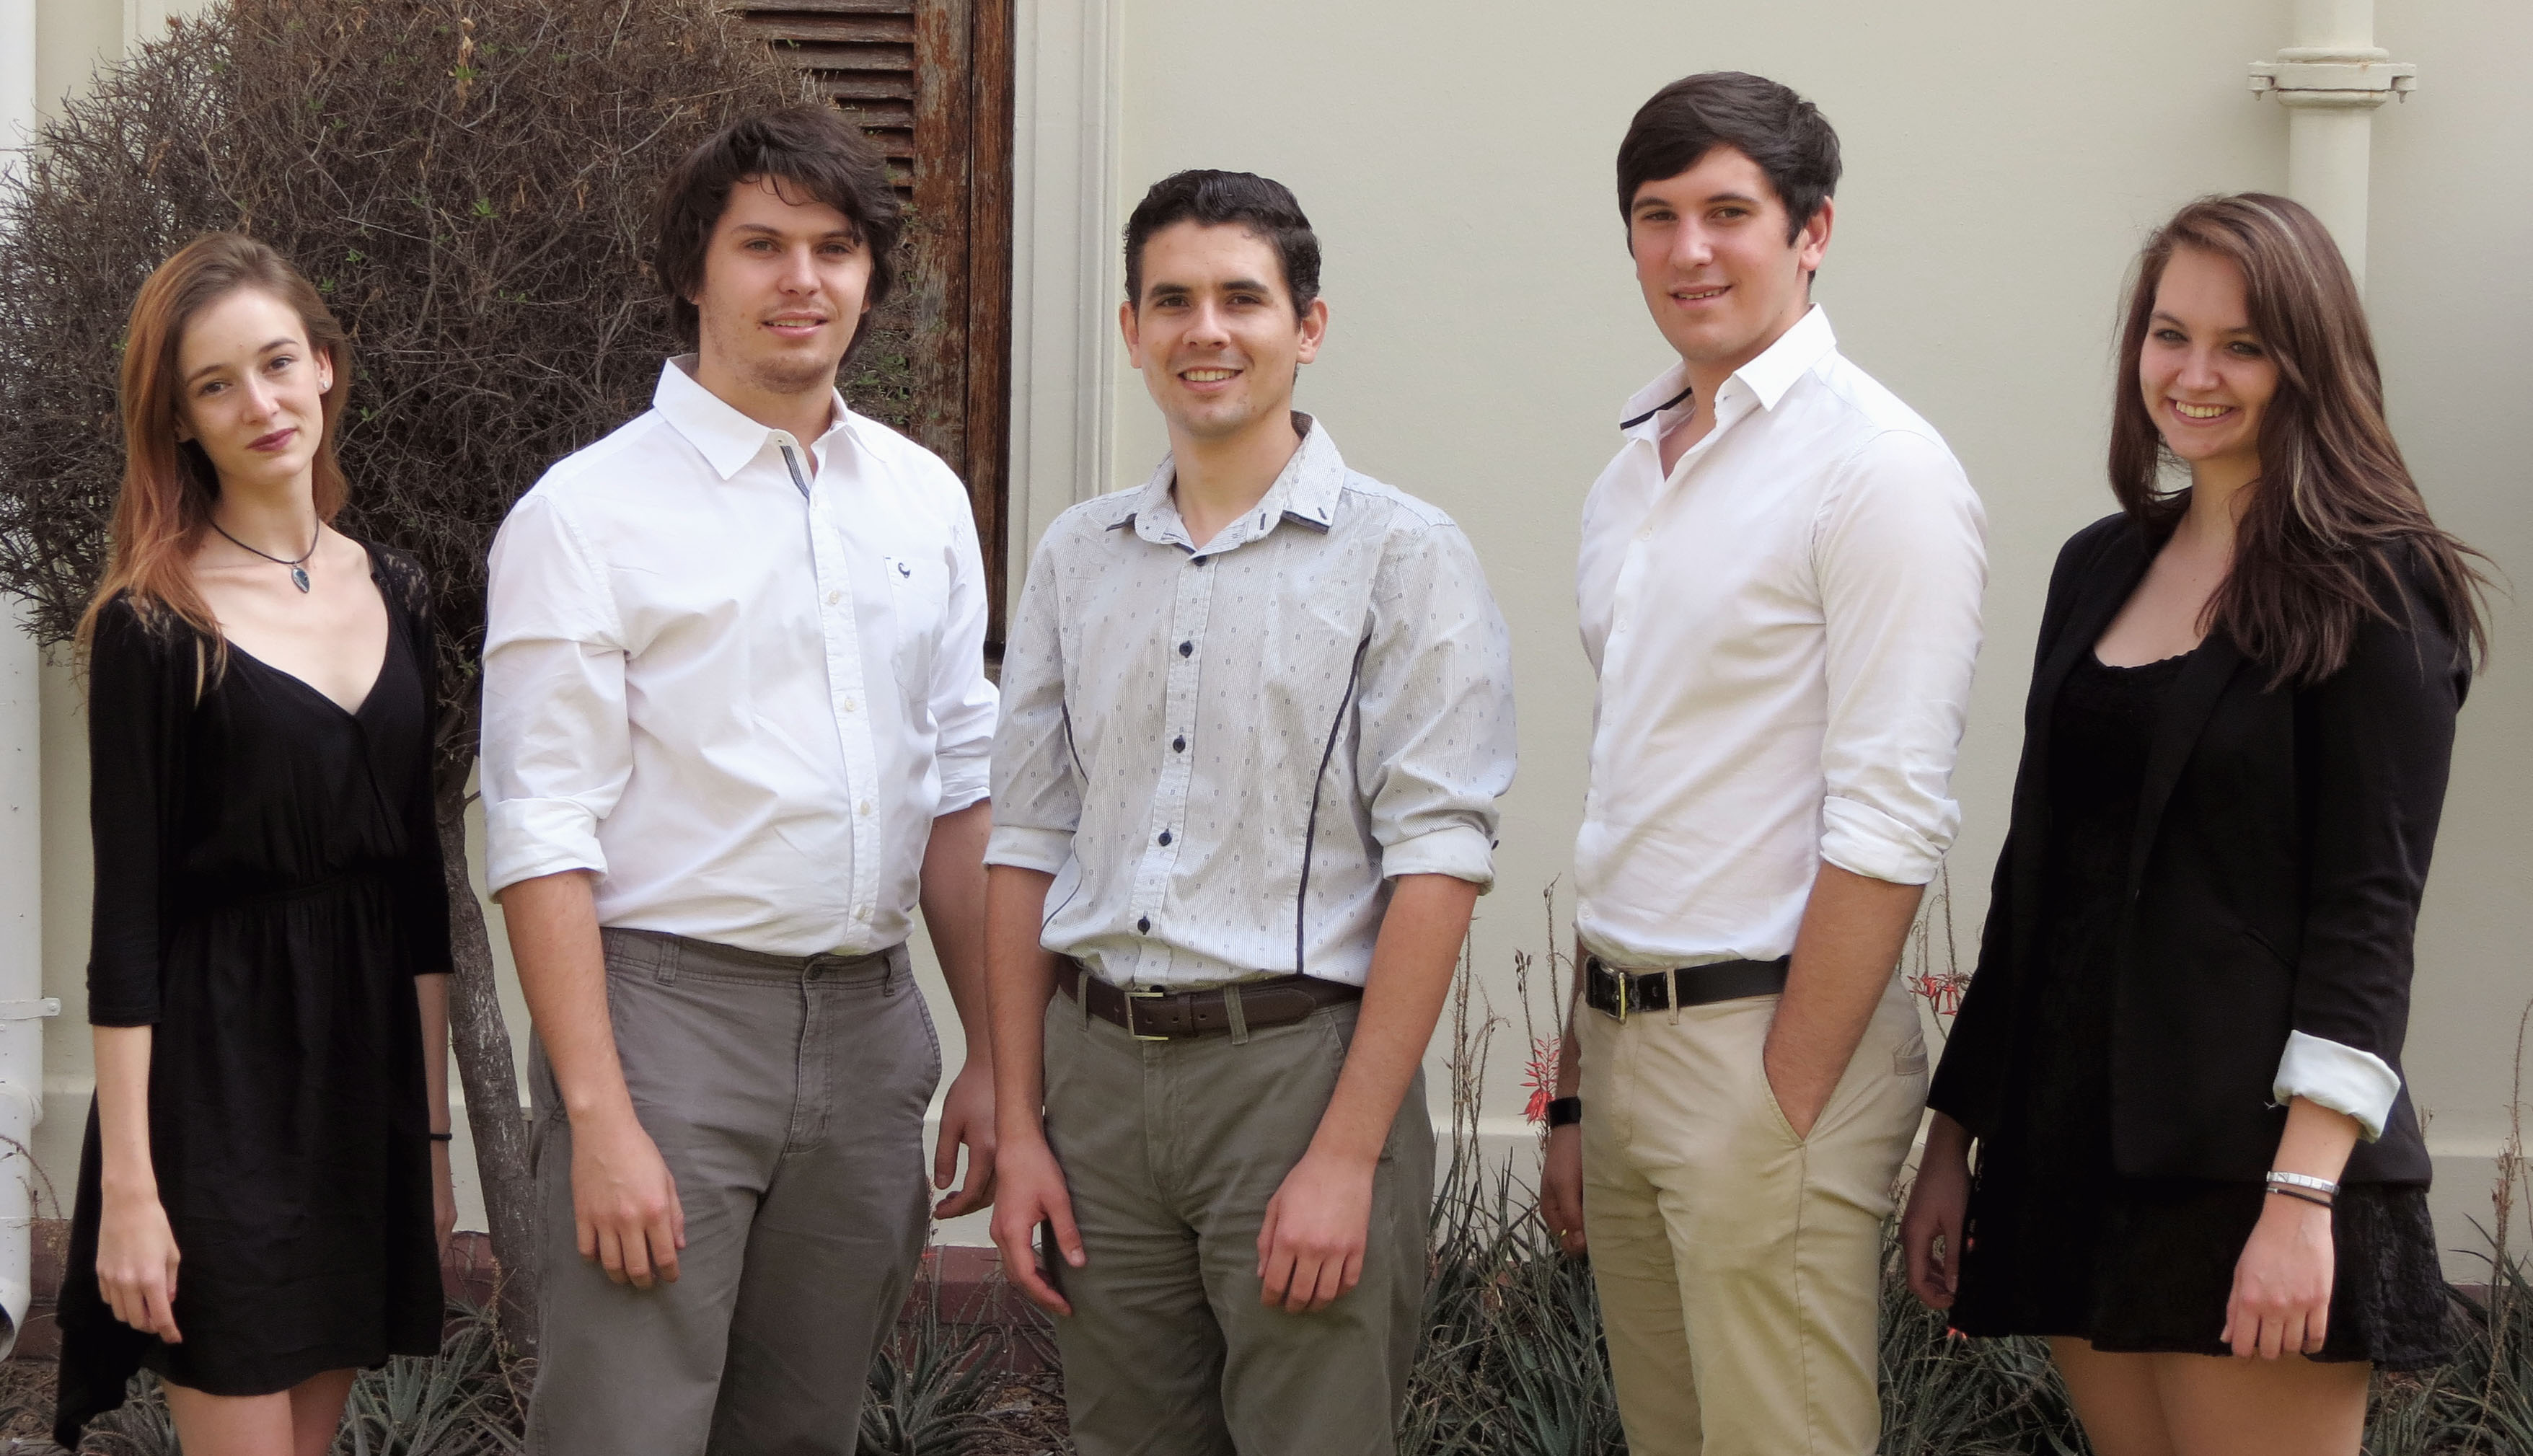
\includegraphics[width=0.5\linewidth]{team.jpg}
\end{center}

\begin{center}
	\large
	\textbf{Mia Gerber}
	\\
	\textbf{Matthew Perry}
	\\
	\textbf{Wanrick Willemse}
	\\
	\textbf{Duart Breedt}
	\\
	\textbf{Linda Potgieter}
\end{center}
\newpage

	\section{Team members (from left to right):}
	\begin{itemize}
		\item \textbf{Mia Gerber}
		\\
		\textnormal Short personal summary
		\\
		\textbf{\small Relevant skills:}
		\begin{itemize}
			\item skill 1
			\item skill 2
			\item skill 3
		\end{itemize}
		
		
		\item \textbf{Matthew Perry}
		\\
		\textnormal Short personal summary
		\\
		\textbf{\small Relevant skills:}
		\begin{itemize}
			\item skill 1
			\item skill 2
			\item skill 3
		\end{itemize}
		
		\item \textbf{Wanrick Willemse}
		\\
		\textnormal Short personal summary
		
		\textbf{\small Relevant skills:}
		\begin{itemize}
			\item skill 1
			\item skill 2
			\item skill 3
		\end{itemize}
		
		
		\item \textbf{Duart Breedt}
		\\
		\textnormal Short personal summary
		\\
		\textbf{\small Relevant skills:}
		\begin{itemize}
			\item skill 1
			\item skill 2
			\item skill 3
		\end{itemize}
		
		
		\item \textbf{Linda Potgieter}
		\\
		\textnormal Short personal summary
		\\
		\textbf{\small Relevant skills:}
		\begin{itemize}
			\item skill 1
			\item skill 2
			\item skill 3
		\end{itemize}
		
		
	\end{itemize}
	
\begin{center}
	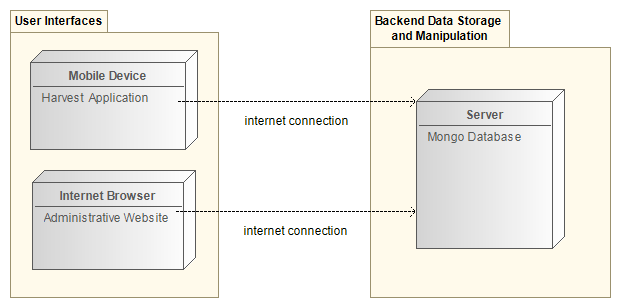
\includegraphics[width=0.5\linewidth]{deployment.png}
\end{center}

\newpage

\large \textbf{Interaction between development team and client:}

\textnormal First and foremost, we believe the client to be the expert, we are merely helping to create
			a system to supplement their already existing domain knowledge. In the case of Subtrop, domain knowledge will consist of typical work hours for farm workers, size of orchards, seasonal influences on crop yields and so forth, which will be acquired during our first meeting if our team is chosen for your project.
			\\ \\
			Moving more into the realm of software engineering, as a team we plan on strictly adhering 
			to Agile Principles. Clients will not only be queried for information but involved as much
			as possible in the testing of early prototypes so that their feedback can be integrated and 
			used as a guide for future releases.
			\\ \\
			Lastly, it is important to us that we as developers and you as our client at Subtrop both 
			agree on a scope for the project, requirements can and probably will change but in order
			to provide the best quality product in the time-frame given we need to first create a checklist of features to be implemented and continually refer back to them to ensure we are not going off scope.
				

\large \textbf{Interaction between members of development team:}

\textnormal We decided on applying a SCRUM methodology in order to structure how teamwork will occur for
			this project, this is a faster, more intensely iterative approach to controlling workflow.
			We are using Slack and ZenHub (in conjunction with Github) to ensure that team members are aware of each other even when we are not physically together and are alerted when work is either available or completed.
			\\ \\
			Meetings will be held once a week regardless of whether there is a problem with
			the project or not, each meeting will require that each team member give a small summary
			of what work they had done that week, this enforces accountability. Working in weekly "sprints" also optimizes predictability and minimizes risk (if something does go wrong it is only a week's worth of work lost, not a whole month)
			\\ \\
			As a team we are going to be adhering to a practice called "pair-programming" which is essentially two or more people working on the same piece of code or feature in order to maximize the chances of bugs being discovered and minimize the time required to get a feature ready for production. 
			\\ \\ 
\end{singlespace} % Uncomment for single line spacing

%----------------------------------------------------------------------------------------

\end{newlfm}
\end{document}
